\startfirstchapter{Introduction}
\label{chapter:introduction}


In this thesis, we consider solving the   problem of localizing a single radiating source based on range and range-difference measurements. The purpose of this chapter is to introduce the systems and methods developed for the problem at hand, discuss the motivations for improving the existing methods, and describe the main contributions and structure of the thesis.

\section{Introduction to Localization Problem} \label{problem}

Geolocation is a rapidly growing field due to the large impact it has on daily life.  The general public has become increasingly dependent on it for realtime navigation, particularly on mobile smartphone devices. Location-based services are  playing an increasingly important role in other fields such as teleconferencing, wireless communications, surveillance, and geophysics \cite{SmithAbel, ShcauRob, Yao, Huang, CheungChan, LiHu, Cheung, Sayed, classMDS}.

Different technologies have been used to build geolocation systems. Several global navigation satellite systems that are available for both military and civilian use and include GPS(US), Galileo(EU), GLONASS(Russia), BeiDou(China). Satellites are equiped with atomic clocks that provide a high-accuracy timing signal to  allow a receiver to calculate the time that it takes the signal to reach the receiver. This information is used to calculate the position of the receiver by using a  computational technique known as trilateration. The location of the receiver can be calculated from the
tracked positions of the satellites and the times measured, each known as the Time-of-Arrival (TOA) \cite{GeoLoc}.
%Consequently, it
%has been incorporated into many services and applications. Currently, outdoor
%localization, thanks to GPS, has revolutionized navigation-based applications running on automotive GPS-enabled devices and smart phones. Applications range from location awareness, to point-by-point directions between destinations, to identifying the closest cinema or coffee shop. The success of GPS has been due to the reliability, availability, and practical accuracy that the system can deliver; however, GPS lacks coverage indoors and in urban areas, in particular near buildings when the signal is blocked;
%even in the best of conditions, the accuracy is on the order of several meters. 
%navigation:
%auto
%aerial
%ships and boats
%heavy equipment
%fitness trackers (for example, Garmin gps enabled smart watches for tracking the run distance/routes/speed)
%
 GPS is widely used in navigation of vehicles such as airplanes, ships, and heavy equipment. It has also been used for monitoring movements rather than navigating, for example in fitness trackers such as FitBit \cite{FB} and Garmin\cite{Garmin} which automatically collect data about the user's activities (distance run, speed, routes taken).
 

As location-based services are becoming increasingly integrated into daily life  the demand for more accurate and robust localization technologies, including in GPS-denied areas, has incresed. One of the approaches to the problem was integration of various wireless technologies with GPS. One such solution is called Assisted GPS (A-GPS), which distributes data and processing over a network of cellular towers equipped with GPS-enabled servers \cite{AGPS}. This can greatly reduce the search space and time to first fix on location. Other systems were built purely on cellular signals, adapting the TOA techniques originally developed for GPS. However their accuracy was limited in urban environments due to obstruction of signals by buildings, and the technique did not gain widespread use beyond the Emergency-911 system it was developed for in the United States.

% Paper: http://www.cs.columbia.edu/~drexel/CandExam/Geolocation_assistedGPS.pdf

With the proliferation of smartphone devices and the internet, WiFi access points are becoming increasingly widespread, providing another means of determining location. One type of WiFi-based technique is called Received Signal Strength (RSS) location fingerprinting. It uses a database of WiFi signatures (RSS values and MAC addresses) with associated GPS coordinates. This has to be built up ahead of time, for example by surveying a city with a GPS and WiFi enabled vehicle. 
Realtime location of the mobile device is determined using the pattern-matching technique, that compares the measured RSSs between the mobile device and access points, and the RSS values stored in the database. Skyhook Wireless successfully developed such system that delivers accuracy of tens of meters in urban areas \cite{Skyhook}. 

Design of any localization system naturally includes a trade-off between the overall performance and cost requirements. Some of the systems developed so far take advantage from the knowledge of the surrounding infrastructure such as
cell towers, Wi-Fi hot spots, or installed RF tags \cite{GeoLoc}. Usually, the precision of the localization in such systems depends on the infrastructure. For example,  hundreds or thousands of meters for cellular survey-based techniques, tens to hundreds of meters, or less than 100 meters for cellular triangulation techniques.

%\textbf{indoor loc - 1 paragraph}

Indoor environments have additional challenges such as limited coverage, multipath signal fading and NLOS conditions. At the same time, indoor applications typically require greater accuracy due to the smaller spaces involved. Robotics was one early application area \cite{Durant}. Systems such as CISCO Wireless Location Application \cite{CiscoWLA} have applied RSS fingerprinting to indoor positioning, which works well if it is possible to install the required infrastructure, and if accuracy on the order of several meters is suffcient. To achieve more accuracy researchers shifted their focus to TOA-based techniques and NLOS mitigation algorithms. Ultra-Wideband communications were used which increase bandwidth and help prevent multipath signal fading \cite{AlaviUWB}.

Combining sensor data from multiple sources to improve localization results is another active area of research. Simultaneous Localization and Mapping (SLAM) is one such technique. The algorithm generates a map of the environment using RF signal, inertial sensors, images, Light Detection and Ranging (LIDAR) and sonar. A topological map is produced which can be used for navigation.

%Developing algorithms to effectively fuse sensor data from multiple sources to
%produce improved localization results is a hot research topic. One popular tech-
%nique is Simultaneous Localization and Mapping (SLAM). SLAM relies on data
%from multiple sensors to build a map of the environment that enables one to
%navigate for long periods of time by using the map to provide location corrections.
%SLAM systems use RF and inertial sensors as well as sensors that measure the
%environment directly such as image, Light Detection and Ranging (LIDAR), and
%sonar sensors to construct a geometric or topological map of the environment and
%then use that map for navigation. The environmental sensors help to alleviate some
%of the problems faced by inertial and RF techniques, but they have their own set of
%problems and challenges in the path to accurate mapping and localization.

%Indoor environments typically hinder wireless propagation because there is uneven coverage and many obstacles. Challenges include the NLOS conditions that 
% Overcoming these physical limitations is the fundamental challenge in indoor localization. As a result, research has shifted back to TOA techniques, while using Ultra-wideband signals which use less power and increase the chance of propagating signals around obstacles.
%
%\textit{The accuracy in the range of tens of meters achieved by techniques described in this section are sufficient for many outdoor applications, but for indoor applications greater accuracy is typically required due to the smaller spaces. If errors of several meters are tolerable, and it is possible to install additional infrastructure, there are existing products such as the CISCO Wireless Location Application \cite{CiscoWLA} which uses RSS fingerprinting. However, this is not sufficient for many envisioned applications so indoor localization remains a very active area of research. Potential applications include tracking children and the elderly in care facilities, tracking inventory and equipment, and tracking personnel in emergency situations. Each application has different requirements for accuracy and reliability.}





\section{Basics of Localization Systems}

Many different systems have been developed for solving the localization problem in different domains such as geolocation, indoor positioning, sonar, etc. Despite the fact that the  solutions themselves are different, they share some fundamental concepts. Classical non-survey based localization systems  are generally comprised of two subsystems: range/angle estimation subsystem and lateration/
angulation subsystem \cite{GeoLoc}. The range/angle estimation subsystem determines distance or direction between the  mobile object of unknown location  and an array of reference points with known location  either pre-programmed or obtained through GPS.  The reference points can be satellites in GPS technology, or base stations in cellular localization, or a set of iBeacons, etc. Lateration/angulation subsystem uses the coordinates of the reference points and the distance or angle estimates to determine the unknown position.  The accuracy of the positioning depends on the accuracy of the anchor nodes’ position, the quality of the range/angle estimates, network geometry, and the performace of the localization algorithm. Figure \ref{fig:2step} describes this two-step procedure.


\begin{figure*}[h]
\centering
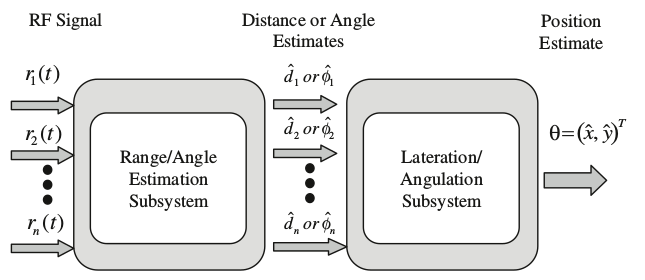
\includegraphics[width=1.0\textwidth]{figures/localization_example.png}
\caption{Classical geolocation system. Range or angle information is extracted from received RF signals. Location is then estimated by lateration/angulation techniques \cite{GeoLoc}.}
\label{fig:2step}
\end{figure*}


In the rest of the section we will provide an overview of the most popular ranging localization methods: TOA, TDOA, AOA, and RSS.



\subsection{Time of Arrival }

Time of Arrival (TOA) localization is a part of class of range-based localization techniques and is often reffered to as tri-lateration. It uses the fact that knowing the propagation speed of  signals between a mobile device and reference points and by measuring the time that a signal takes to be received, the distance can easily be calculated. To obtain an $n$  dimentional position estimate at least $n+1$ range measurements are required. Note that absolute times are used in calculations, so it is critical that the  clocks in base stations and the mobile device are synchronized. It is also assumed that they are all in LOS condition. %Unfortunately, this is not always the case in practice. %In many situation this is not practicle.

Solution techniques developed for range-based localization can be grouped under Maximum Likelihood (ML) and Least Squares (LS) approaches. 
Given the observed range measurements $\Br_n = \Br + \Bw$, the ML estimate $\hat{\Bx}$ of the unknown source location $\Bx$ is obtained by maximizing the conditional probability density function 
\begin{equation}
\nonumber
\hat{\Bx} = \mbox{arg}\max_{\Bx} P\left(\Br_n|\Bx\right)
\end{equation}
where $\Bw$ represents measurement noise. One of the major problems with ML approach is that it requires the knowledge of exact error-free measurements. Another difficulty is that solving for the unknown position extimate is computationally difficult. Many variants and approximations of the original ML has been  developed \cite{Guvenc}, \cite{Guvenc2}, \cite{HoML}.

In LS approaches the source location extimate $\hat{\Bx}$ is found by minimizing the sum of risiduals \cite{GeoLoc}
\begin{equation}
\nonumber
\hat{\Bx} = \mbox{arg}\min_{\Bx} \left\lbrace \sum_{i=1}^m \beta_i\left(r_n^{(i)} - \|\Bx - \Ba_i\|\right)^2 \right\rbrace
\end{equation}
where $a_i$ is a vector of known coordinates of reference points (sensors),   $r_n^{(i)}$ is a range measurement associated with it, $\beta_i$ is a weight
that can be used to emphasize  the degree of confidence in the measurement, and $m$ is a number of sensors.


\subsection{Time Difference of Arrival}

\subsection{Angle of Arrival}

Localization using angle-of-arrival is simpler than time-based techniques in that
only two angle measurements are required, as opposed to three range measure-
ments, in order to estimate the two-dimensional position. However the challenge is
presented when obtaining accurate angle of arrival estimation using wireless
devices. In typical scenarios, the base stations are equipped with K antenna array
elements spaced by D which are capable of estimating the angle of arrival which is
then used to locate the mobile device. Figure 2.4 illustrates the basic concept of AOA localization. The relationship between the coordinates and the angles is given by

The performance of AOA positioning techniques in LOS conditions is satis-
factory. However, in severe NLOS multipath conditions the reliability and accu-
racy of AOA techniques suffers considerably. As a result in these unfavorable
propagation conditions, TOA- or RSS-based techniques are preferred. Further-
more, hybrid positioning techniques can be used to incorporate the advantages of
two different techniques which usually outperform the individual techniques.


\begin{figure*}[h]
\centering
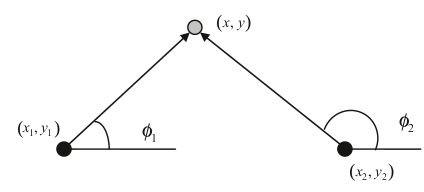
\includegraphics[width=0.7\textwidth]{figures/angle_of_arrival.png}
\caption{AOA positioning (angulation). The AOA estimate from 2 base stations to the mobile terminal can be used to estimate the position \cite{GeoLoc}.}
\label{fig:2step}
\end{figure*}


\subsection{Received Signal Strength}



%\subsection{Old}
%
%Review of ranging and localization methods, theory behind it, application, limitations. 
%
%TOA,
% 
%TDOA,
%
%AOA ?,
%
%non-range-based? 
%
%"Geolocation techniques"
%
%\cite{GeoLoc}
%\cite{LiuSurvey}

\section{Contributions and Organization of the Thesis}

\subsection{Contributions  of the Thesis} \label{contributions}


single source localization

something like:

the material developed here / mathematical tools and methods are suitable for many different scenarios 
OR
can have different world life applications, for example: TOA, TDOA, static positioning using UWB range measurements. 

This work mostly investigated possible localization solution for the wireless sensor networks that use radio frequency measurements to obtain the range or range-difference measurements. However, some of the methods presented in this work can also be applied for other mediums, i.e. ultrasonic, sonic, light. 

In this paper, which considers both problems, the main focus is on efficient computation of least squares (LS) estimates of the source’s coordinate vector. The models that we consider for the said vector are based on  the assumption that the sensor network can be used, along with some form of preprocessing, to obtain (noisy) range or range-difference measurements. From a practical standpoint, this is a simplifying assumption (e.g., in nonline-of-sight scenarios), albeit one commonly made in \cite{Cheung} and \cite{classMDS} ([7] and [8]). Even so, the resulting location estimation problems are nonconvex and, therefore, rather difficult to solve globally, which explains why only approximate solutions to them have appeared in \cite{SmithAbel}, ~, \cite{LiHu} ([1], [2], [5],) and \cite{Cheung}. We should also mention here the family of data fusion methods \cite{Sayed} in which linear least squares problems are constructed via subtraction of equations. However, these methods do not provide optimal solutions since they implicitly assume the existence of an error-free measurement. In this paper, we first consider the problem of source localization from range measurements. 


In Section II we provide a result that explains why a recently proposed semidefinite relaxation (SDR) \cite{Cheung} of the R-LS approach to this problem may yield an accurate approximation; however, we also show that the SDR may lead to a poor approximation. For lack of a good solution to the R-LS problem, we then turn our attention to an SR-LS approach. Although the latter approach also leads to a nonconvex problem, we show that this problem can be efficiently and globally solved. Then we go on to consider the source localization problem from range-difference measurements in Section III. Our main results here concern an SRD-LS approach to this problem. In particular, we show that despite the fact that the said SRD-LS problem is also nonconvex, it can be efficiently solved, and we provide the details of an algorithm that computes the global solution of this problem. We end Section III by remarking that an SDR approach applied to a corresponding RD-LS criterion leads to extremely poor solutions. Several numerical examples suggest that the exact SR-LS and SRD-LS solutions can be more accurate by several orders of magnitude than existing approximate SR-LS and SRD-LS estimates, and than SDR-based approximations of the R-LS and
RD-LS solutions.

\subsection{Organization of the Thesis} \label{organization}

\begin{description}
\item[\textbf{Chapter 1}] contains a statement of
the claims which will be proved by this dissertation followed by an overview of the structure of the document itself. Describes in details the open problem which is to be tackled together with its context, its impact and the overall motivation for the research overall.
\item[\textbf{Chapter 2}] IRW-SR-LS.
\item[\textbf{Chapter 3}] PCCP.
\item[\textbf{Chapter 4}] Sequential Relaxation.
\item[\textbf{Chapter 6}] contains a restatement of the claims and results of the dissertation. It also enumerates avenues of future work for further development of the concept and its applications.
\end{description}